% \documentclass{standalone}
%  \input{../tikz_header.tex}
 
%  \begin{document}
 


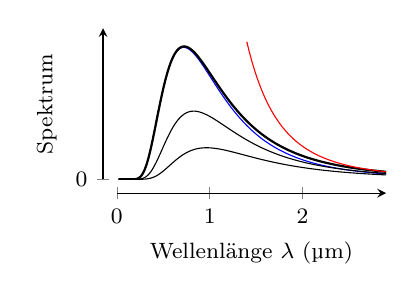
\begin{tikzpicture}[font=\footnotesize
%declare function={ 	  },
]
%\useasboundingbox (0,0) rectangle (5,5);
%\draw (0,0) rectangle (5,5);

\begin{axis}[no markers, 
	samples=150,
    %      ymin=-0.3, ymax=1,
      xmin = 0., xmax = 2.9,
    ymin = 0, ymax = 4,
      %  axis y line=left,
       %    axis x line=bottom,
          %xtick = {0,1},
          %xticklabels= {0, $\pi/a$},
      %     xticklabels = {\footnotesize $R_g$, \footnotesize $R_e$},
         ytick = {0},
         %  yticklabels = { , $1/2$, , $3/2$, , $5/2$, , $7/2$, , $9/2$, , $11/2$},
        %ytick = {0,1},
         %  yticklabels = { 0, $ \sqrt{\frac{4 \, c_1}{M}}$},
            xlabel = {Wellenlänge $\lambda$ (\textmu m) },
        ylabel = {Spektrum},    
        %x label style={at={(axis description cs:1, 0)},anchor=north east, yshift=-7pt},
    %y label style={at={(axis description cs: 0,1)},anchor=south east,  yshift=10pt},
           width= 5cm, height = 3.5cm,
  separate axis lines,
  axis x line=bottom,
  axis x line shift=5pt,
  %xlabel shift=10pt,
  axis y line=left,
  axis y line shift=5pt,
%  ylabel shift=10pt           
           ]
           
           %  \frac{8 \pi h \nu^3}{c^3} \,  \frac{1}{e^{\frac{h \nu}{k_b T}} -1} \, d\nu 
           
        % x = lambda in um ; 1/x = nu   ; 1/x^2 wg nu -> lambda

        \addplot [domain=0:3,  thin, blue]    { 100 * (1/x)^5 *   exp(-0.01439*10^6 / (x * 4000)) };


        \addplot [domain=0:3,  thick]    {100 * (1/x)^5  / (exp( 0.01439*10^6 / (x * 4000)) -1)};
        \addplot [domain=0:3,  thin]    {100 * (1/x)^5  / (exp( 0.01439*10^6 / (x * 3000)) -1)};
        \addplot [domain=0:3,  thin]    {100 * (1/x)^5  / (exp( 0.01439*10^6 / (x * 3500)) -1)};
 

        \addplot [domain=1.4:3,  thin, red]    {100 * (1/x)^4   * 0.14};


 

 \end{axis}

\end{tikzpicture}


%\end{document}